\documentclass[12pt]{article}%
\usepackage{amsfonts}
\usepackage{fancyhdr}
\usepackage{comment}
\usepackage[a4paper, top=2.5cm, bottom=2.5cm, left=2.2cm, right=2.2cm]%
{geometry}
\usepackage{times}
\usepackage{amsmath}
\usepackage{changepage}
\usepackage{amssymb}
\usepackage{graphicx}%
\usepackage[UTF8]{ctex}
\usepackage{hyperref}
\usepackage{appendix}
\usepackage{listings}
\setcounter{MaxMatrixCols}{30}
\newtheorem{theorem}{Theorem}
\newtheorem{acknowledgement}[theorem]{Acknowledgement}
\newtheorem{algorithm}[theorem]{Algorithm}
\newtheorem{axiom}{Axiom}
\newtheorem{case}[theorem]{Case}
\newtheorem{claim}[theorem]{Claim}
\newtheorem{conclusion}[theorem]{Conclusion}
\newtheorem{condition}[theorem]{Condition}
\newtheorem{conjecture}[theorem]{Conjecture}
\newtheorem{corollary}[theorem]{Corollary}
\newtheorem{criterion}[theorem]{Criterion}
\newtheorem{definition}[theorem]{Definition}
\newtheorem{example}[theorem]{Example}
\newtheorem{exercise}[theorem]{Exercise}
\newtheorem{lemma}[theorem]{Lemma}
\newtheorem{notation}[theorem]{Notation}
\newtheorem{problem}[theorem]{Problem}
\newtheorem{proposition}[theorem]{Proposition}
\newtheorem{remark}[theorem]{Remark}
\newtheorem{solution}[theorem]{Solution}
\newtheorem{summary}[theorem]{Summary}
\newenvironment{proof}[1][Proof]{\textbf{#1.} }{\ \rule{0.5em}{0.5em}}

\newcommand{\Q}{\mathbb{Q}}
\newcommand{\R}{\mathbb{R}}
\newcommand{\C}{\mathbb{C}}
\newcommand{\Z}{\mathbb{Z}}

\begin{document}

\title{人工智能 实验报告:模拟退火算法}
\author{熊永琦 16340258}
\date{\today}
\maketitle

\begin{center}
本项目所有代码均已在 \href{https://github.com/xwy27/ArtificialIntelligenceProjects}{小组 Github 仓库} 开源
\end{center}

\section{实验要求}

在 TSPLIB(http://comopt.ifi.uni-heidelberg.de/software/TSPLIB95/,多个地址有备份;其他网站还可以找到有趣的 Art TSP 和 National TSP)中选一个大于100个城市数的 TSP 问题,完成如下要求:

\begin{enumerate}
\item 采用多种邻域操作的局部搜索 Local Search 策略求解
\item 在局部搜索策略的基础上,加入模拟退火 Simulated Annealing策略,并比较两者的效果
\item 要求求得的解不要超过最优值的10%,并能够提供可视化,观察路径的变化和交叉程度
\end{enumerate}

\section{局部搜索:爬山算法}

\subsection{爬山算法原理}

作为一种启发式算法,爬山算法的思想很简单:从当前解集出发,寻找一个领域空间内的所有解,通过估价函数求得他们的估价,然后根据这个估价寻找到最优解,再从最优解重新开始执行算法。

爬山算法的优点在于其收敛迅速,因其只会沿着到当前估价下降(假设估价最低的为最优解)最快的方向选择解(如果临域算法足够好),且不会有回退的情况出现。

其缺点往往也非常明显:经典的爬山算法无法处理局部最优解,一旦到达一个局部最优,或者说函数曲线上的极点,其就会无法继续求得更优的解。而在一些情况下,局部最优解和全局最优解相去甚远。因而单纯通过爬山算法求得的解有时候会甚至没有办法作为近似解使用。

\subsection{临域操作设计}

在本项目中,我们使用一个节点序号数组来维护当前解,也就是销售员走的路径,其中开头和末尾固定为节点 1。我们一共为爬山算法设计了四种临域操作:

\begin{enumerate}
    \item 随机选择两个节点,交换其在队列中的位置
    \item 随机选择三个节点,轮换其在队列中的位置
    \item 随机选择两个节点,使得其间的节点次序反向
    \item 完全随机生成一个路径序列
\end{enumerate}

其中,在每个循环中,我们都通过每条规则分别生成 1000 个可能解。通过上述算法,我们在每次循环中都为其生成了一个规模为 4000 的可行解集。然后,我们将在其中找出拥有最优估价的可行解,并使用这个解作为起点,继续进行爬山算法,直到迭代次数达到上限为止。

\section{模拟退火算法}

\subsection{模拟退火算法原理}

模拟退火算法顾名思义,模拟的是现实中冶金专家为了达到某些特种晶体结构重复将金属加热或冷却的过程。这种算法为避开局部最优,达到全局最优而生。它在系统朝着能量减小的趋势这样一个变化过程中,偶尔允许系统跳到能量较高的状态,以避开局部极小点, 最终稳定到全局最小点。

更形象地讲,它可以理解为一个「允许接受更坏解」的爬山算法,通过这样允许不那么好的解被接受为下一跳的起点,它能够跨过山脊,从一个山峰跳到另一个山峰,并通过降温(限制更坏解被接受的概率),最终收敛到相对更高的山峰上。

\subsection{临域操作的修改}

在爬山算法中,我们每次循环都使用了一个多达 4000 可行解的解集,但是这在模拟退火算法中是没有必要的。在爬山算法中,我们需要尽可能地覆盖函数曲线上的临域,来达到离散模拟连续量的效果,而模拟退火是通过随机跳转实现这一过程的,因而我们将其缩减了一千倍,每种算法仅提供一个可能解。

\subsection{温度变化曲线和参数的选择}

在每个内层循环中,我们对四种临域算法生成的解分别进行一次尝试,然后进行一次降温。我们使用现有温度 * 0.9999849 作为我们的下一个温度,这个函数的曲线起初下降迅速,然后下降缓慢,比较符合现实中高温物体的温度变化,同时从逻辑上讲,这种降温曲线让我们的算法在前期寻找到较好山峰后能集中精力攀登更高峰。

在参数选择上,经过测试,我们最终选定的初始温度为 1850,外循环次数为 40000 次。

\section{测试与结论}

\subsection{数据选择与最优解}

我们选择 KroA150 作为测试数据集,该数据集合内包含了 150 个城市,满足题目要求。其最优解的路径长度为 26524\cite{besttsp}。

\subsection{测试结果}

我们分别在进度为约 50\% 时和进度达到 100\% 时采集了数据,结果如下:

\ 

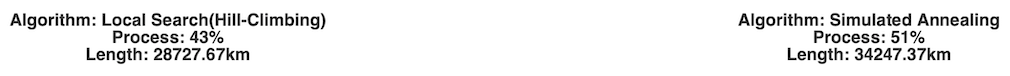
\includegraphics[width=\textwidth]{mid.png}

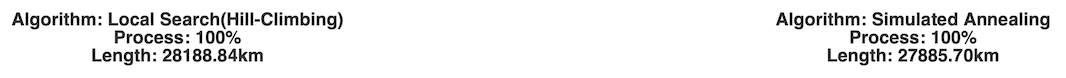
\includegraphics[width=\textwidth]{final.png}
\begin{center}
    FIGURE 1. 50\% 和 100\% 进度时结果
\end{center}

其中,左侧均为局部搜索(爬山)算法,右侧均为模拟退火算法,Process 为当前算法迭代完成进度,Length 为当前选定路径的路径长度。我们通过调整参数,使得两个算法的完成速度相近。

\subsubsection{局部搜索}

我们可以看到,局部搜索迅速收敛到了一个较优解(28727.67),但是在之后57\%的过程中,其几乎都在原地踏步,最终收敛在了 28188.84,是最优解的 1.06 倍。

\subsubsection{模拟退火}

模拟退火算法一开始收敛速度并不快,甚至会有些时候在开倒车(Length 变大),直到进度到达 51\% 时,其 Length 不过到了 34247.37,是爬山算法的 1.2 倍。但是在之后的 49\% 进度中,它不断进步,最后收敛到了 27885.70,这个结果为最优解的 105\%,比爬山法减少了 400 的 Length。

\subsection{对比与总结}

在优秀的临域算法设计和参数选择下,两种算法都成功地跑进了最优解 10\% 的范围内,但是他们呈现出的特点依旧是截然不同的。

爬山算法拥有非常惊人的速度,在进度不到一半的时候,已经获得了一个很好的解(最优解10\%以内),但是在之后给其的大多数计算资源被白白浪费了——他并没能在优秀的基础上更进一步。

模拟退火算法并不在意短时间去获得一个一般的解,它更倾向于用时间去打磨一个更优的解。在算法初期,高温使得各种质量的解都能被接受(当然,优秀的解有更大概率被接受),随着温度下降,算法逐渐倾向于只接受好解,并最终收敛到一个更高的山峰上。你可以从图 1 中看到,模拟退火实际上以更短的时间求得了一个更优的解。在避开局部最优解的问题上,模拟退火做得很不错。尤其是当你有更充裕的时间时,你可以通过调节降温速度、初温等手段来充分利用多出来的时间,而爬山算法却只能在一个小山丘上眼巴巴地看着你往上爬。

总的来说,如果用户对于解的质量要求不高,爬山算法能在最短时间内给出一个能够接受的解;而模拟退火会尽它所能给你一个更接近最优解的答案,当然,相对的,模拟退火的耗时可能会更长。

\begin{thebibliography}{}
\bibitem{besttsp} https://www.iwr.uni-heidelberg.de/groups/comopt/software/TSPLIB95/STSP.html
\end{thebibliography}

\end{document}